\chapter{SOM input type study}

\label{chap:som-fv-cifar}

In this chapter, we show analysis of SOM performance and results with two types of input. Both setups use the same dataset - CIFAR-10 dataset, but they differ in type of preprocessing of the data. First setup use CIFAR-10 datasetet with no preprocessing. In second setup, the CIFAR-10 dataset is preprocessed in such way, that we used Mean teacher model with properly chosen hyperparameters that provide state-of-the-art performance of the model and calculate feature vectors of each input sample. Mean teacher model was trained with $4000$ labeled samples, other samples were unlabeled. Feature vectors (FV) are representations from output of last convolutional layer in MT model. We compared these two setups to show, that feature vectors of MT model are suitable for SOM to learn the original dataset representation. And they lead to even better topology of SOM than vanilla dataset.

\section{Experient description}
Task in this experiment was clustering of 10 classes. Dataset CIFAR-10 was already described in section \ref{dataset-cifar10}. It is image dataset with 10 classes. 
In first setup, we used this dataset as it is. For the second setup, we trained Mean teacher model. We used implementation by CuriousAI\footnote{https://github.com/CuriousAI/mean-teacher}, which is original implementation, which was used, when MT was published by Tarvainen in \cite{tarvainen}. In the repository, readme says, it is possible to achive model with reported results by running script $\texttt{cifar10\_test.py}$. We did that and saved parameters of the model, which achieved accuracy $93.68\%$ (student) and $93.88\%$ (teacher). Feature vectors were produced by student model weights. 

For both trainings - with CIFAR-10 and with feature vectors - we used the same implementation of SOM and hyperparameters as described in section \ref{pretrained-som}. We investigated several SOM sizes and provided further investigation of SOM metrices (quantization error, winner discrimination and entropy), as well as the map visualization.



\section{Results}
We investigated som sizes from $6\times6$ to $15\times15$ neurons in map .
Each SOM was trained for $100$ epochs. The training curves of SOM metrices are shown in figure \ref{fig:cifar-6n-99ep-stat} and figure \ref{fig:fv-6n-99ep-stat}. In figure \ref{fig:cifar-6n-99ep-stat} we can see the change of metrices during whole training for $6 \times 6$ map with vanilla CIFAR-10 input. In figure \ref{fig:fv-6n-99ep-stat} we can see the same metrices for $6 \times 6$ map with feature vectors input. 
 Graphs look very similar in their behavior for all SOM sizes in the same input type setup. There is difference between one setup and another. Quantization error has different trend. In FV setup, it looks more nonlinear, in CIFAR-10 setup trend looks linear. In entropy, CIFAR-10 has increasing direction during first $80$ epochs and then it drops a little. Entropy in FV setup has very chaotic progress during first $60$ epochs, then it increase relatively quick and reach similar values as in CIFAR-10 setup. Winner discrimination is in all cases and during whole training $100\%$, which means, all neurons are chosen as winner for some input. It is reasonable, since number of inputs is large.

\begin{figure}[h!]
    \centering
    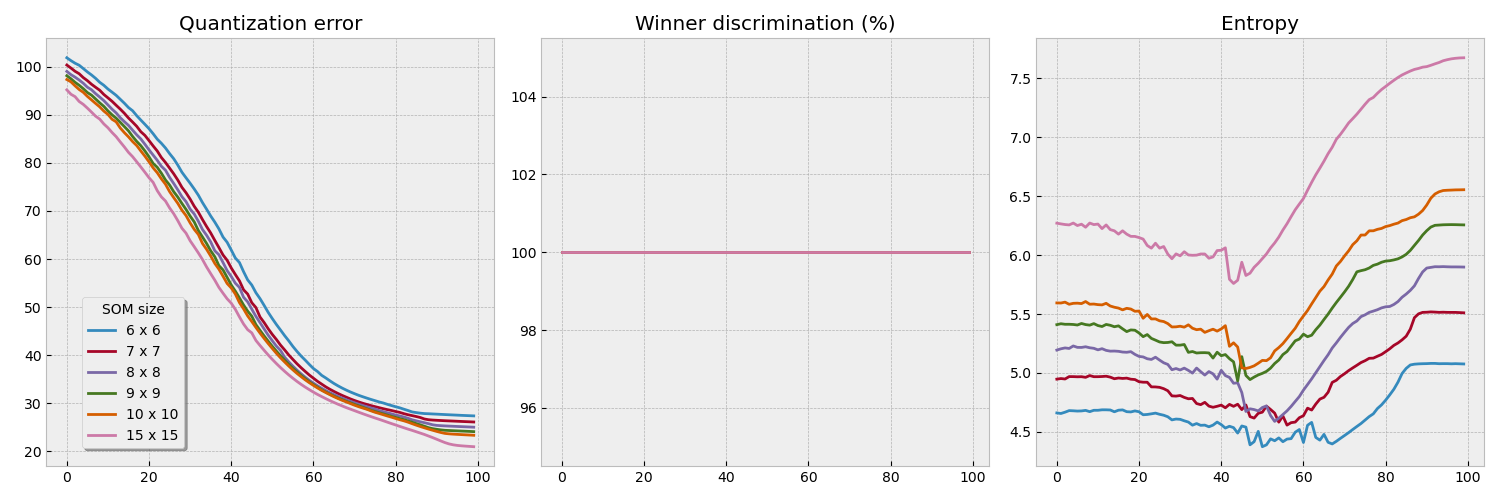
\includegraphics[width=1\textwidth]{figs/fv-som-measures.png}
    \caption{FV input: SOM metrices change during 100 tr. epochs}
    \label{fig:fv-6n-99ep-stat}
\end{figure}

\begin{figure}[h!]
    \centering
    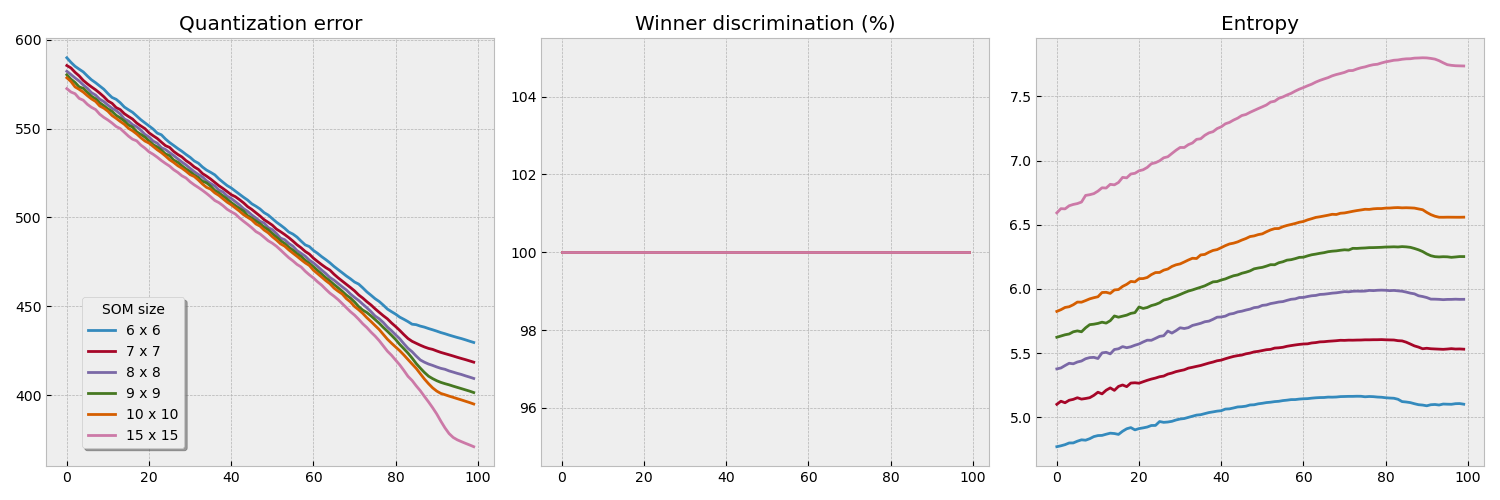
\includegraphics[width=1\textwidth]{figs/cifar-som-measures.png}
    \caption{CIFAR-10 input: SOM metrices change during 100 tr. epochs}
    \label{fig:cifar-6n-99ep-stat}
\end{figure}


For both setups entropy reached the peak arround epoch $85$. Quantization error also start decrease slower after circa $85$ epochs. Since by qualitative metrices this looks as moment with the best performance of the SOM, we look further in metrices and  visualization of the map at this moment of training in following sections.

\subsection{SOM metrices after 85 epochs}

In this section, we provide data of SOM metrices after $85$ epochs for investigated SOM sizes. Results are shown in table \ref{tab:som-metrices-85ep}. We can see, that in all cases, winner discrimination is $100\%$, which means, all neurons are chosen as winner during training process. Entropy in both setups for one chosen size does not differ that much, but we can see, that for CIFAR-10 inputs, SOM entropy is a little higher. When it comes to quantization error, for feature vector approach, it is much lower, so the prototypes and inputs has smaller average distance in $n$-dimensional space, then in opposite approach. 

\begin{table}[h!]
\centering
\begin{tabular}{|c|rrr|rrr|}
\hline
\multicolumn{1}{|l|}{} & \multicolumn{3}{c|}{FV from MT}                                              & \multicolumn{3}{c|}{CIFAR 10}                                            \\ \hline
\multicolumn{1}{|c|}{map size} & \multicolumn{1}{c|}{QE} & \multicolumn{1}{c|}{WD} & \multicolumn{1}{c|}{E} & \multicolumn{1}{c|}{QE} & \multicolumn{1}{c|}{WD} & \multicolumn{1}{c|}{E} \\ \hline
6 $\times$ 6& \multicolumn{1}{r|}{28.17}   & \multicolumn{1}{r|}{100.0\%}   &  5.0 & \multicolumn{1}{r|}{439.87} & \multicolumn{1}{r|}{100.0\%} &  5.12 \\ \hline
7 $\times$ 7& \multicolumn{1}{r|}{27.41}   & \multicolumn{1}{r|}{100.0\%}   &  5.28 & \multicolumn{1}{r|}{430.24} & \multicolumn{1}{r|}{100.0\%} &  5.6 \\ \hline
8 $\times$ 8& \multicolumn{1}{r|}{26.54}   & \multicolumn{1}{r|}{100.0\%}   &  5.64 & \multicolumn{1}{r|}{424.38} & \multicolumn{1}{r|}{100.0\%} &  5.98 \\ \hline
9 $\times$ 9& \multicolumn{1}{r|}{26.04}   & \multicolumn{1}{r|}{100.0\%}   &  5.98 & \multicolumn{1}{r|}{420.8} & \multicolumn{1}{r|}{100.0\%} &  6.33 \\ \hline
10 $\times$ 10& \multicolumn{1}{r|}{25.73}   & \multicolumn{1}{r|}{100.0\%}   &  6.29 & \multicolumn{1}{r|}{417.47} & \multicolumn{1}{r|}{100.0\%} &  6.63 \\ \hline
15 $\times$ 15& \multicolumn{1}{r|}{24.34}   & \multicolumn{1}{r|}{100.0\%}   &  7.53 & \multicolumn{1}{r|}{408.19} & \multicolumn{1}{r|}{100.0\%} &  7.79 \\ \hline

\end{tabular}
\caption{SOM metrices after 85 training epochs}
\label{tab:som-metrices-85ep}
\end{table}

\subsection{Map visualization after 85 epochs}
In this section, we show visualization of SOM maps after $85$ epochs of training. We choose SOM with size $10\times10$ neurons, to show qualitative difference of results of two input types. Maps are visualized in figure \ref{cifar10-fv-85ep}. On this figure, color of the neuron represents for which class this neuron was chosen as winner most frequently, while size of the neurons represents percentage of inputs from this major class from all inputs that chose this neuron as their winner - prototype.

\begin{figure*}[h!]
    \centering
    \begin{subfigure}[t]{0.4\textwidth}
        \centering
        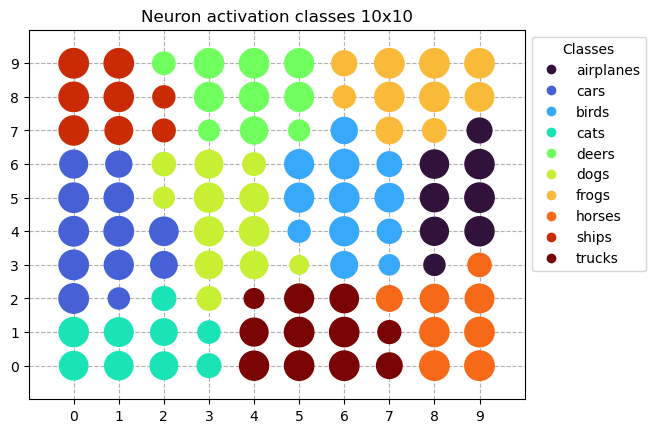
\includegraphics[height=2.2in]{figs/fv-10n-84ep.png}
        \caption{FV input: SOM map visualization}
    \end{subfigure}%
    ~ 
    \begin{subfigure}[t]{0.6\textwidth}
        \centering
        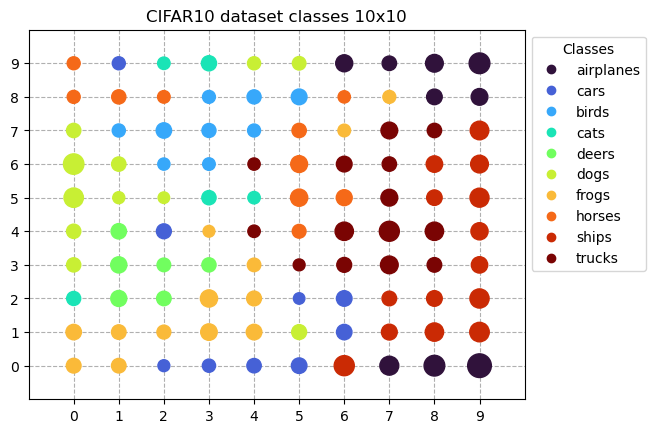
\includegraphics[height=2.2in]{figs/cifar10-10n-84ep-new.png}
        \caption{CIFAR-10 input: SOM map visualization}
    \end{subfigure}

    \caption{Comparison of maps with FV input and CIFAR-10 input}
    \label{cifar10-fv-85ep}
\end{figure*}


On the left side, we can see SOM that was trained from feature vectors of Mean teacher model. On the right side, there is SOM trained from unmodified CIFAR-10 dataset. We can see, that clusters on the left map are completely one from another, but on tre right side, there are some clear clusters on the right part and in the down left corner of the map, but in the centre, there are outlayers and disconnected groups of neurons from the same class. Maps differ also in neuron sizes. Since on the left map, prototypes are huge, which means, they properly encode inputs from one class and not many inputs from other classes, in the right map, sizes are very small, so prototype encode more than one class. Based on this visual investigation of map organizations, we can infer that FV input type improve clustering ability of SOM.


\subsection{SOM neuron weights visualization}
Since SOM neurons are prototypes of inputs and the similarity to input is hidden in neuron weights, which has the same size as input vectors, in vanilla CIFAR-10 input setup, we can visualize weights as images. If neuron properly represents a class of inputs, we should see some shapes typical for this object in the image. We trained $10 \times 10$ SOM in the same way as before, and visualize its map and weights after $100$ epochs in figures \ref{fig:som-for-weights} and \ref{fig:som-weights}.

\begin{figure}[h!]
    \centering
    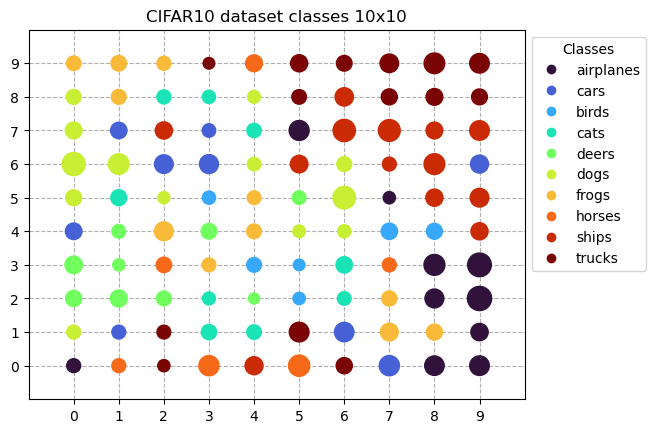
\includegraphics[width=0.6\textwidth]{figs/saved-cifar10-10n-99ep.png}
    \caption{SOM used for weight visualization, map after 100 epochs}
    \label{fig:som-for-weights}
\end{figure}

We can see, that map is not organised well, there are many outlayers, even though we can see some visible clusters of trucks, ships, airplanes, that cover almost all inputs from the class. When it comes to weight visualization, most of the prototypes does not look like specific object from one class, however, there are few of them, that look like car, truck, horse or frog. Other classes are not that evidently visible on the visualization.


\begin{figure}[h!]
    \centering
    \includesvg[width=1.0\textwidth]{figs/from-som-weights-10n-99ep.svg}
    \caption{$10 \times 10$ SOM weights visualization}
    \label{fig:som-weights}
\end{figure}


\section{Discussion}
From this study, we can infer, that using feature vectors as the input of Self-organizing map is adventageous in few ways. First, SOM map has better qualitative results, that means smaller quatization error. Second, also qualitative result - visualization - shows better distribution of data into clusters and less outlayers. And last, since the feature vectors representation has lower dimension than the original inputs, training lasts less time. Based on these observations, we decided to use feature vector inputs in our semi-supervised model with auxilary SOM loss.

